\documentclass[11pt]{article} % For LaTeX2e
\usepackage{nips12submit_e,times}
%\documentstyle[nips12submit_09,times,art10]{article} % For LaTeX 2.09

\usepackage[utf8]{inputenc}
\usepackage[T1]{fontenc}
\usepackage{textcomp}
\usepackage[scaled=0.8]{beramono}

\usepackage{caption}
\usepackage{subcaption}
\usepackage{amsmath,amssymb}
\usepackage{booktabs}
\usepackage[pdftex]{graphicx}
\usepackage{color}

\usepackage{url}
\usepackage{hyperref}

\newcommand{\todo}[1]{\noindent\texttt{\color[rgb]{0.5,0.1,0.1} TODO: #1}}

\title{Simulating disease spread in social networks\thanks{Final project
for the course ``Introduction to Social Network Analysis'' (Spring
Semester 2012).}}

\author{
Alkis Gkotovos\\
Department of Computer Science, ETH Zurich\\
\texttt{alkisg@student.ethz.ch}
}

\nipsfinalcopy % Uncomment for camera-ready version

\begin{document}

\maketitle

\begin{abstract}
In this report I present a model, similar to the common SIR and SIS models,
which can be used to simulate the spread of an infectious disease in
social networks. I also present and discuss simulation results on several
kinds of generated networks for different choices of model and graph parameters.
\end{abstract}

\section{Introduction}
The spread of diseases in human networks is an interesting research topic, both
for historical reasons (e.g. analysis of the ``Black Death'' pandemic in the
14th century~\cite{blackdeath}), as well as for dealing with contemporary or
future epidemics (e.g. AIDS spread in Africa~\cite{aids}). Furthermore, the
concept of network diffusion can be generalized to other types of phenomena,
like the spread of computer viruses in e-mail networks~\cite{email}, or even
the spread of behavioral phenomena, also referred to as
\emph{social contagion}~\cite{contagion}.

To fully analyze disease spread in networks, one needs to know in detail the
characteristics of the disease itself (transimission, active period, etc.),
as well as a fine-grained network of interactions. Moreover, the network
information required may depend on the disease attributes (e.g. for an airborne virus
it may be important to include interactions in public transport). Since this
kind of information is usually not available, there have been proposed a
number of simple models that can be used as a first step for analyzing disease
spread. Two of them, commonly found in the literature, are the SIR and SIS
models~\cite{easley, newman}.

Both models assume discrete time steps and represent each node of the network
as a state machine that can be in exactly one state at each time step. In the
SIR model healthy nodes that can be infected are in the \emph{susceptible} ($S$)
state, infected nodes are in the \emph{infected} (I) state, and nodes that have
gone through the infection and cannot be infected again are in the \emph{removed}
($R$) state. At every time step, an $I$ node may independently infect each of
its $S$ neighbors with probability $p_I$ and an $I$ node stays infected for
$t_I$ steps and, afterwards, transitions into the $R$ state.
The SIS model is very similar and only differs in the fact that nodes return
to the $S$ state after the infection is over, instead of transitioning to the
$R$ state.

\section{Model description}
I introduce a new disease spread model, called SIMR, which is very similar to
the SIR/SIS models, albeit slightly more complex. The rationale behind extending
these models is twofold. First, the SIR/SIS models only allow transitions out
of the $I$ state after the whole infectious period has passed, which I find to be
constraining, because it defines a completely fixed period that a node will be
infected. Second, in choosing one of the two models, one has to stick with
always transitioning to either the $S$ state or the $R$ state, after the infection
is over, which I also find inflexible.

With the above ideas in mind, the SIMR model works as follows:
\begin{itemize}
\item As in the SIR/SIS models, healthy nodes are in the $S$ state and infected
nodes are in the $I$ state. Also, as before, an $I$ node may infect any of its
$S$ neighbors with probability $p_I$.
\item The first extension is that, although an $I$ node stays infected for $t_I$
time steps, it can transition to the $R$ state with probability $p_R$ at each
time step of the infection. This, in a sense, models the fact that an infected
person may pass away at any point during the infected period with a certain
probability.
\item The second extension is that the transition after the infection is over
is not fixed, but is determined probabilistically. In particular, the previously
infected node transitions to an \emph{immune} ($M$) state with probability $p_M$,
or otherwise returns to the $S$ state. The $M$ state is the same with the $R$
state from an operational perspective, but is semantically different.
\end{itemize}

\section{Simulation}
In this section I first present three popular types of randomly generated
networks and briefly discuss their characteristics. Then, I use generated
graphs from these classes to simulate the SIMR model for various combinations
of graph and SIMR parameters.

\subsection{Random graph models}
\noindent\textbf{Erdős–Rényi model.} The Erdős–Rényi (ER) model~\cite{erdos} is
probably the simplest possible model for generating a random graph. The
construction process of the graph consists in specifying the number of
nodes $n$ and, subsequently, independently adding every possible edge
with probability $p$. We expect that the notion of \emph{percolation
threshold}, i.e. the value of $p$ that, for given $n$, differentiates
between a single large graph component and a number of small graph
components, plays an important role in disease spread. I will refer to a
generated graph of this class as ER$(n, p)$.

\noindent\textbf{Watts-Strogatz model.} The Watts-Strogatz (WS)
model~\cite{watts} was proposed as a more realistic model for generating graphs
that have \emph{small-world} properties, i.e. large clustering combined with
short average path lengths. The graph is constructed by starting with a ring
topology of $n$ nodes, where each node is connected to its $k$ closest neighbors
in the ring. Subsequently, every existing edge is rewired withe probability $p$.
We expect that disease spread will be more severe in such a network, because
of the small-world properties. I will refer to a generated graph of this class
as WS$(n, k, p)$.

\noindent\textbf{Barabási-Albert model.} The Barabási-Albert (BA)
model~\cite{barabasi} aims to generate graphs with \emph{scale-free} degree
distributions, which may be more realistic than the degree distributions of
WS graphs. A graph is generated by implementing the notion of
\emph{preferential attachment}. In particular, for generating a graph with
$n$ nodes, one node is added at a time and it is connected to $m$ of the
existing nodes with probability proportional to the degree of each existing
node. It follows that the model favors the creation of hubs, i.e. nodes that
accumulate a lot of edges, which is expected to play a role in disease spread
(for example, removing a few large hubs from the network might make a huge
difference). I will refer to a generated graph of this class
as BA$(n, m)$.

\begin{figure}[t]
  \begin{subfigure}[b]{0.5\textwidth}
    \centering
    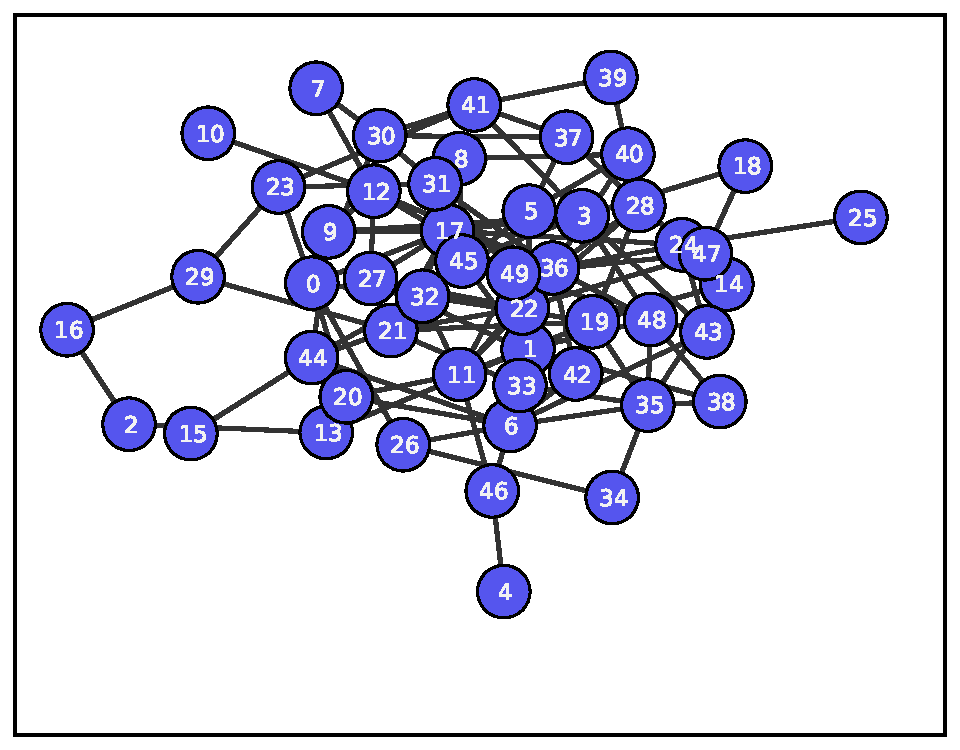
\includegraphics[width=\textwidth]{figures/ER_graph_50_01_init}
  \end{subfigure}
  \begin{subfigure}[b]{0.5\textwidth}
    \centering
    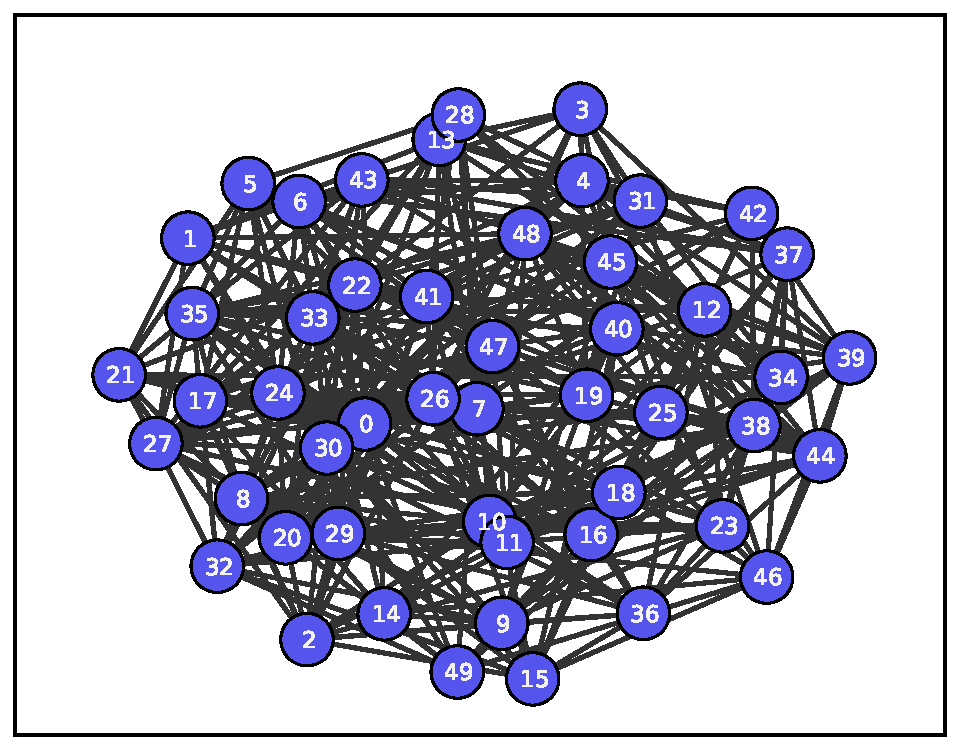
\includegraphics[width=\textwidth]{figures/ER_graph_50_03_init}
  \end{subfigure}
  \caption{An ER(50, 0.1) network (left) and an ER(50, 0.3) network (right).}
    \label{fig:graph_er}
\end{figure}

\begin{figure}[t]
  \begin{subfigure}[b]{0.5\textwidth}
    \centering
    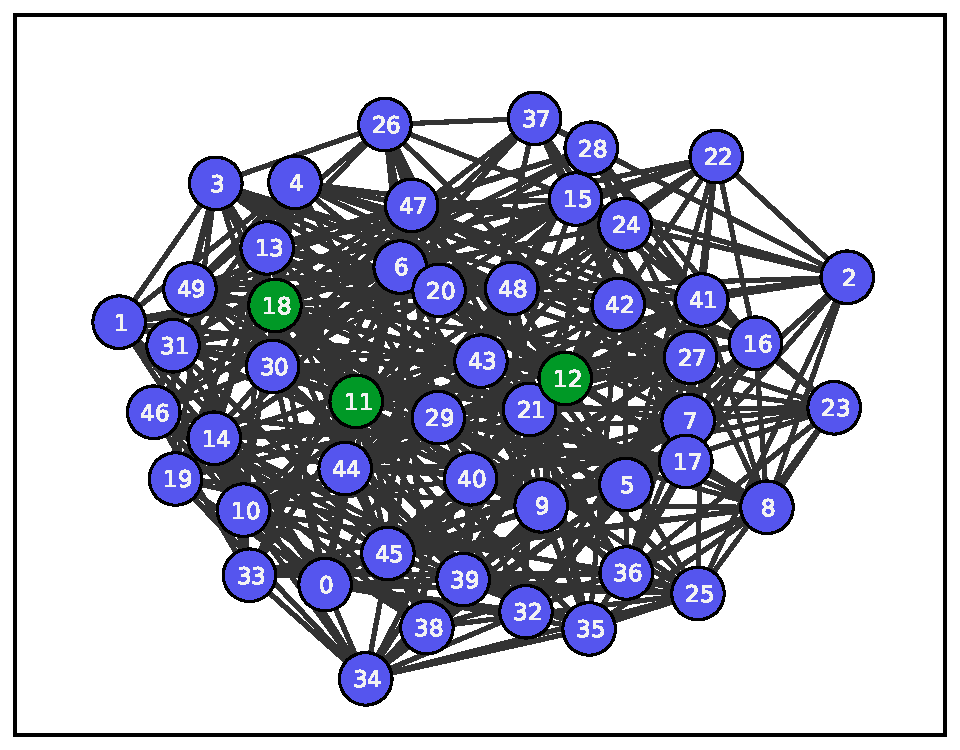
\includegraphics[width=\textwidth]{figures/ER_evo_50_03_init}
    \caption{Initial graph state}
  \end{subfigure}
  \begin{subfigure}[b]{0.5\textwidth}
    \centering
    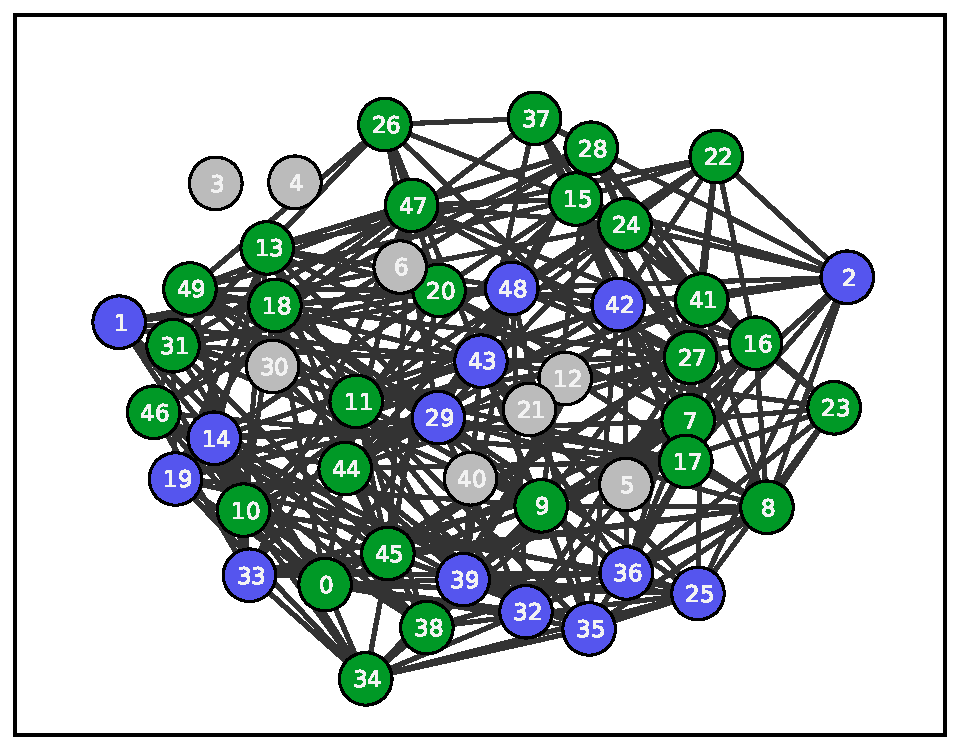
\includegraphics[width=\textwidth]{figures/ER_evo_50_03_10}
    \caption{Graph state after 10 steps}
  \end{subfigure}
  \begin{subfigure}[b]{0.5\textwidth}
    \centering
    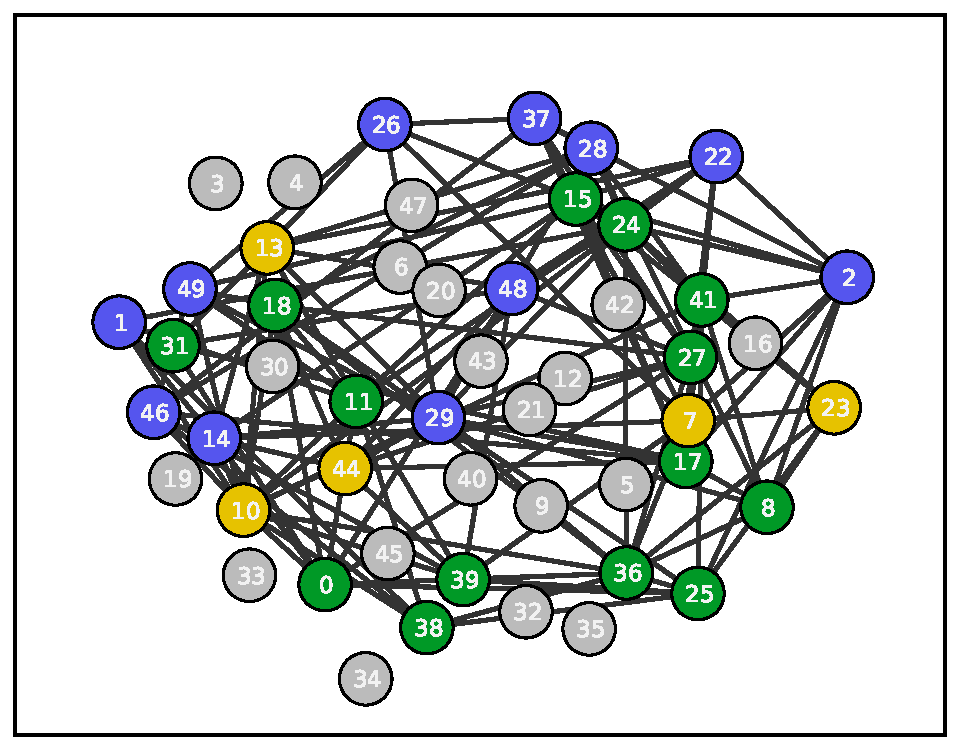
\includegraphics[width=\textwidth]{figures/ER_evo_50_03_20}
    \caption{Graph state after 20 steps}
  \end{subfigure}
  \begin{subfigure}[b]{0.5\textwidth}
    \centering
    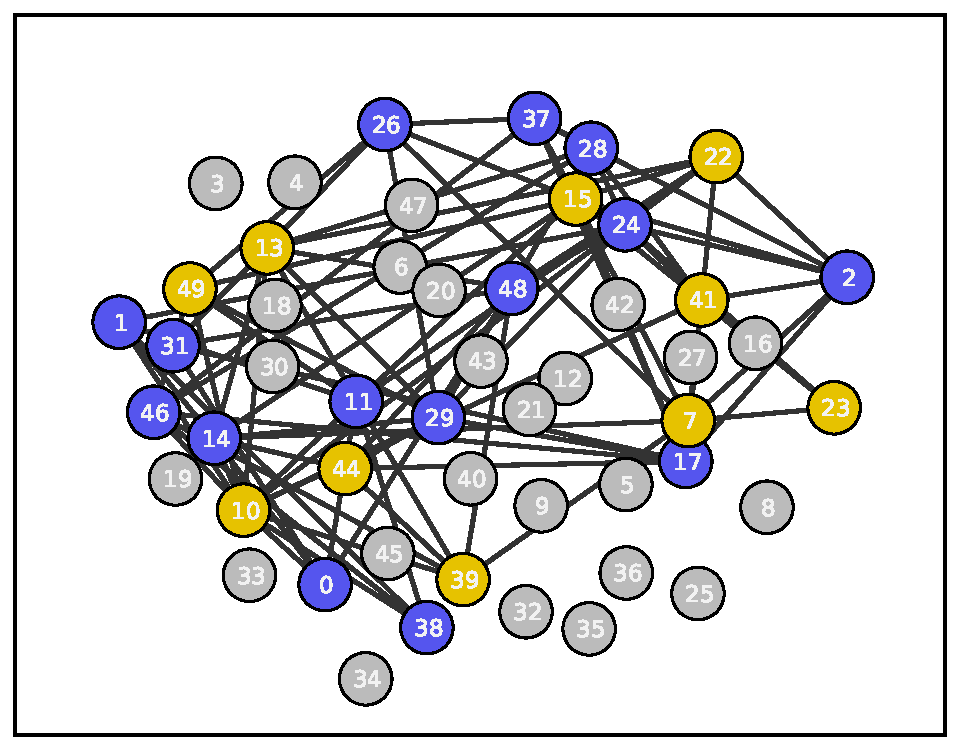
\includegraphics[width=\textwidth]{figures/ER_evo_50_03_final}
    \caption{Final graph state}
  \end{subfigure}

  \caption{States of the ER(50, 0.3) graph of Figure~\ref{fig:graph_er}}
    \label{fig:graph_evo_er}
\end{figure}

\begin{figure}[t]
  \centering
  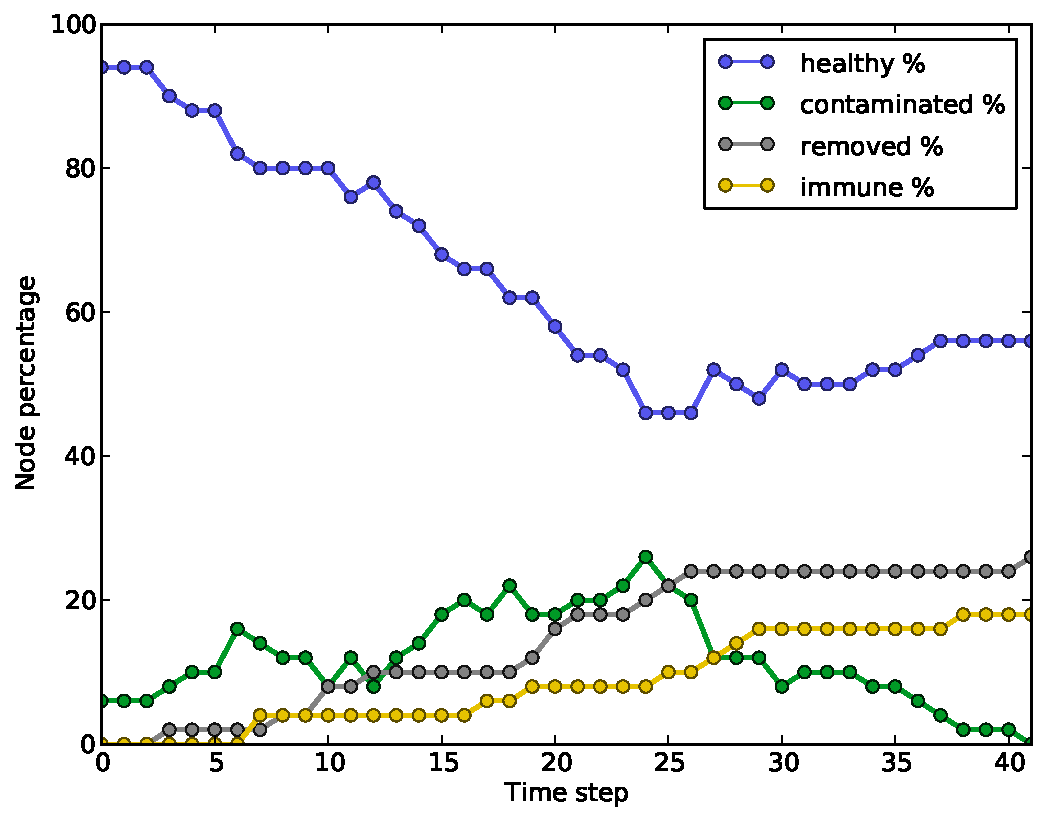
\includegraphics[width=0.49\textwidth]{figures/ER_evo_50_01}
  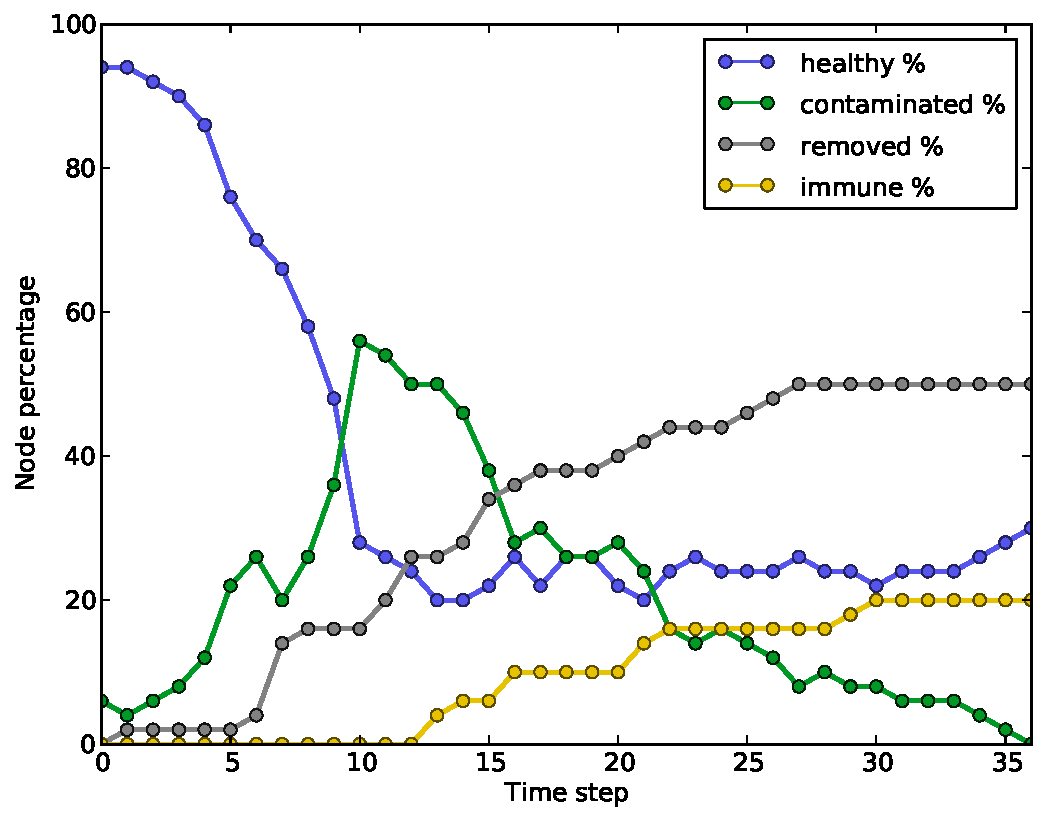
\includegraphics[width=0.49\textwidth]{figures/ER_evo_50_03}
  \caption{Evolution plots for the graphs of Figure~\ref{fig:graph_er}.}
    \label{fig:evo_er1}
\end{figure}

\begin{figure}[t]
  \centering
  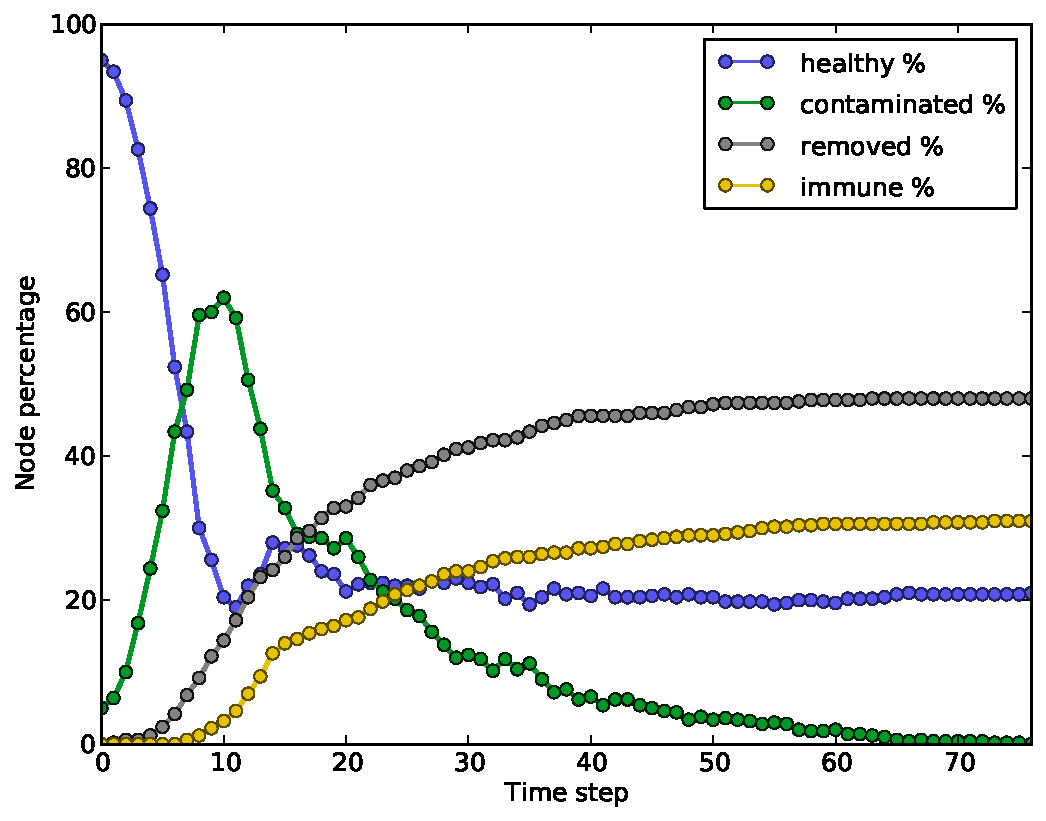
\includegraphics[width=0.49\textwidth]{figures/ER_evo_500_003}
  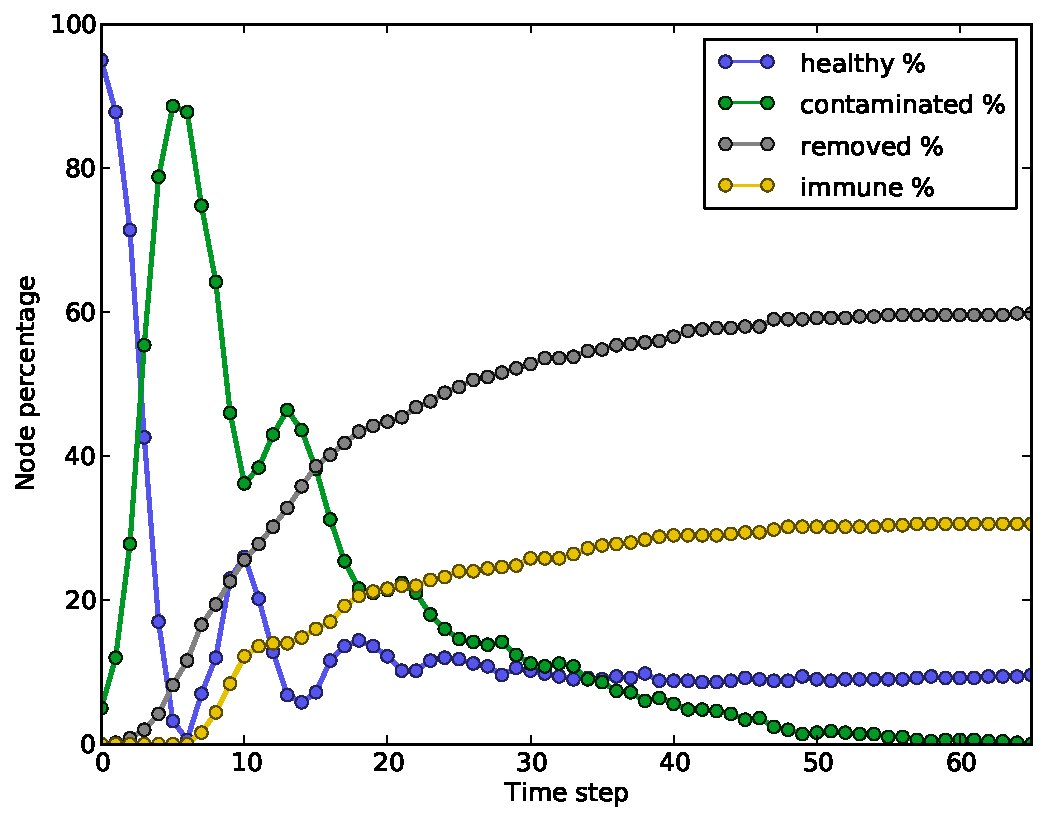
\includegraphics[width=0.49\textwidth]{figures/ER_evo_500_007}
  \caption{Evolution plots for an ER(500, 0.03) graph of (left) and an
    ER(50, 0.03) (right).}
    \label{fig:evo_er2}
\end{figure}

\bibliographystyle{plain}
\bibliography{report}

\end{document}
